\documentclass[11pt,a4paper]{article}
\usepackage[T1]{fontenc}
\usepackage[utf8]{inputenc}
\usepackage{lmodern,microtype}
\usepackage[margin=23mm]{geometry}
\usepackage{amsmath,amssymb,booktabs,array,graphicx,siunitx,xurl}
\usepackage[numbers,sort&compress]{natbib}
\usepackage[colorlinks=true,linkcolor=blue!50!black,citecolor=blue!50!black,urlcolor=blue!50!black]{hyperref}
\usepackage{xcolor,placeins}
\graphicspath{{figures/}}
\newcommand{\dd}{\mathrm{d}}
\newcommand{\code}[1]{\path{#1}}
\newcommand{\Qbb}{Q_{\beta\beta}}
\setlength{\parindent}{0pt}
\setlength{\parskip}{5pt plus 1pt}
\setlength{\emergencystretch}{3em}
\title{ITACA: principle of operation\\Triggered electron and ion readout}
\author{Working design note}
\date{9 November 2026}
\begin{document}
\maketitle
\begin{abstract}
ITACA measures the electrons and positive ions produced by the same ionising
track. Electroluminescence provides the fast energy measurement and electron
track. An accepted energy trigger predicts where and when to collect the ion
track, positions the movable detector and controls a cathode gate. This note
organises the operating sequence, signal formation, readout, signal treatment
and reconstruction of both tracks. The new design uses a configurable drift
field of 300 V/cm at 15 bar and records the CSA output with a 12-bit ADC every
100 microseconds. Digital reconstruction is a separate stage. The operating
choices are design inputs; the ADC, trigger-window prediction and nonlinear
inverse described here are the next implementation. Existing productions
retain their recorded configurations.
\end{abstract}
\tableofcontents

\section{Overall view: one event, two tracks}
\label{sec:overview}
Consider a neutrinoless double-beta event at $(X,Y,Z)$ and time $t_0$.
Its two electrons deposit a total energy near $\Qbb=2458$ keV through an
extended track. Ionisation produces an electron and a positive ion per primary
pair. The relevant positive carrier is the molecular ion $\mathrm{Xe}_2^+$,
of charge $+e$. Primary scintillation supplies $t_0$.

Define $z=0$ at the ELM entrance and $z=L$ at the cathode drift boundary.
Electrons from a deposit at $z$ drift through $z$; its ions drift through
$L-z$. The vertex labels the event, while all its deposits determine the
arrival interval. In a uniform drift region,
\begin{equation}
 t_e(z)=t_0+\frac{z}{v_e},\qquad
 t_i(z)=t_0+\frac{L-z}{v_i}+\delta_i.
 \label{eq:times}
\end{equation}
Here $\delta_i$ is the calibrated travel time through the focusing structure
to the pad. Electron readout timing similarly includes the calibrated delay
of EL emission and electronics.

The electron track, or \emph{etrack}, is measured first. The ion track, or
\emph{itrack}, arrives seconds later with much less diffusion. This delayed
coincidence defines the operating sequence~\cite{itaca2026}:
\begin{enumerate}
\item Record primary scintillation and read the EL signal. Sum its calibrated
response to estimate event energy $E_{\rm fast}$.
\item Accept the energy trigger if
\begin{equation}
 |E_{\rm fast}-\Qbb|\leq\mathrm{FWHM}_E(\Qbb).
 \label{eq:roi}
\end{equation}
The ROI is $\pm1$ FWHM, with full width $2$ FWHM. Its width is expressed in
energy units and calibrated for the fast energy estimator.
\item For accepted events, the fast-trigger algorithm (FTA) estimates the
etrack barycentre, longitudinal and transverse extent and arrival-time
distribution. Together with $t_0$, these predict the ion footprint and arrival
window. Under the MARS design, the movable ion detector is positioned to
contain that footprint, including its uncertainty.
\item Acquire the CSA baseline, open the cathode gate shortly before the
predicted first ions, collect the track, close the gate after its predicted
last ions and finish a short post-arrival recording. Rejected candidates
leave the ion gate closed.
\end{enumerate}
The EL measurement supplies the primary energy estimate; the ion branch is
optimised for topology. Both branches yield reconstructed charge and position
for consistency checks and combined track analysis. The manuscript also
describes a barrel fibre detector for scintillation timing and calorimetry.
The selected fast-energy channel, whether that detector or the calibrated ELM
sum, and its FWHM belong to the trigger configuration.

\subsection{Operating defaults}
\begin{table}[htbp]\centering\small
\begin{tabular}{p{.47\linewidth}p{.43\linewidth}}
\toprule
Quantity & New operating proposal\\\midrule
Chamber length; pressure; gas & 1.5 m; 15 bar; Xe--15\% He\\
Drift field $E_d$ & 300 V/cm\\
Reduced drift field $E_d/P$ & 20 V/cm/bar, derived\\
Electron drift velocity $v_e$ & Approximately 0.6 mm/$\mu$s; graph estimate\\
Maximum electron drift time & Approximately 2.5 ms\\
Ion velocity model & $v_i=\mu_i E_d$, calibrated mobility\\
Ion pitch & 4 mm initially; configurable\\
EL pitch; hole diameter; depth & 4 mm; 2.5 mm; 5 mm\\
EL reduced field & 2 kV/cm/bar initially\\
EL time buckets & 250 ns\\
Ion ADC & 100 $\mu$s; 12 bits; provisional 0--1.8 V\\
Digital voltage averaging & 5 ms initially\\
Stored ADC samples & Compressed HDF5, \texttt{UInt16}\\
Energy ROI & $\Qbb\pm1$ FWHM\\
Gate opening advance & 1 ms before the predicted early boundary\\
\bottomrule
\end{tabular}
\caption{User design choices agreed on 9 November 2026. Cards select geometry,
transport, acquisition and reconstruction independently.}
\label{tab:defaults}
\end{table}
Drift field and pressure are independent card inputs; their ratio is derived.
An explicitly supplied ratio must agree with them. The EL reduced field is a
different parameter applying inside the holes.

At 300 V/cm and 15 bar, $E_d/P=20$ V/cm/bar. Figure 8 of
Ref.~\cite{McDonald_2019} gives approximately $v_e=0.6$ mm/$\mu$s for Xe--15\%
He. This is a graphical estimate transferred by reduced-field scaling from
measurements at 1--9 bar, rather than a direct 15-bar calibration. Therefore
$L/v_e\simeq2.5$ ms is the illustrative maximum drift time. EL formation and
electronics add their response duration. A refined transport calculation or
measurement will supply the gas-, field- and temperature-dependent card value.

The previous ion design used 0.1 m/s at 200 V/cm. Keeping that mobility gives
$\mu_i=5\times10^{-6}$ m$^2$/(V s) and, illustratively, $v_i=0.15$ m/s at
300 V/cm. Maximum ion drift then takes 10 s; a 10--100 mm longitudinal extent
gives approximately 67--667 ms of arrivals. This assumes field-independent
mobility at fixed gas and pressure and requires calibration. One second is an
event-duration scale, not a fixed acquisition length.

A reconstructed time bucket $T_i$ corresponds to $v_iT_i$ along $z$. At this
illustrative velocity, 40 ms represents 6 mm and 4 mm corresponds to 26.7 ms.
ADC sampling, reconstructed bucket width and transverse pitch are separate
choices. Likewise 250 ns corresponds to approximately 0.15 mm for the new
electron velocity. Earlier productions retain their original velocity and
distance-to-time conversions.

\subsection{Predicting when ion acquisition ends}
For inferred undiffused longitudinal extent $[z_{\min},z_{\max}]$, the nominal
collection boundaries are
\begin{equation}
 t_{is}=t_0+\frac{L-z_{\max}}{v_i}+\delta_i,
 \qquad
 t_{ie}=t_0+\frac{L-z_{\min}}{v_i}+\delta_i.
 \label{eq:boundaries}
\end{equation}
The earliest electron deposits correspond to the latest ions. The FTA derives
these boundaries from EL measurements and calibration. Simulation truth
evaluates their accuracy separately.

Diffusion is statistical. For independent, zero-mean displacements, a useful
variance relation is
\begin{equation}
 s_e^2=s_0^2+\langle\sigma_{e,L}^2(z)\rangle+s_{\rm readout}^2,
 \qquad
 s_i^2=s_0^2+\langle\sigma_{i,L}^2(L-z)\rangle.
 \label{eq:widths}
\end{equation}
All terms are expressed in spatial units and consistently charge-weighted,
correcting attachment and channel response. These relations guide a fit to
the longitudinal profile; its endpoints have uncertainties. EL emission,
sensor response and sampling enter $s_{\rm readout}$. The predicted interval
is defined by a specified retained-charge fraction and timing uncertainty.

The gate opens at $t_{is}-m_{\rm early}$ and closes at
$t_{ie}+m_{\rm late}$ after converting pad-arrival predictions to gate-crossing
times. The early margin includes the agreed 1 ms advance and uncertainty
allowance; the end margin covers the late diffusion tail and timing error.
ADC recording starts before opening and ends after the last admitted ions
have crossed the collection structure and the digital filter has finished.
The short post-arrival recording measures the final CSA state, which still
contains accumulated charge.

A gap or weak section of the itrack does not itself end acquisition. Validation
measures excluded charge and endpoint errors as margins are varied. The
three-second post-event recording used in earlier CSA studies remains useful
for selected recovery tests. Ordinary acquisitions use the event-specific
window and short filter-completion interval.

\section{EL signal formation and readout}
\label{sec:el}
Primary-pair sampling is shared between arms. For $\overline N=E/W$, the Fano
prescription is $\operatorname{Var}(N)=F\overline N$. The same realised count
feeds ions and electrons. Integer sampling at small means preserves the mean
and respects the variance allowed for integer counts. Electrons drift,
diffuse and survive attachment with probability $\exp[-t_e/\tau_e]$.
The electron lifetime is configurable, initially 15 ms. Ions receive no
electron-attachment loss.

The ELM focuses electrons into holes. The current optical model assumes unit
electron collection for EL reduced fields at least 2 kV/cm/bar. Mean yield per
entering electron is parameterised as
\begin{equation}
 Y_g=a_g P d[(E_{\rm EL}/P)-b_g],
\end{equation}
with $d$ in cm, $P$ in bar and reduced field in kV/cm/bar. Gas-dependent
coefficients and their provenance are documented in \code{../../docs/elm.tex}
and selected by the detector card. At fixed entering count $N_e$,
\begin{equation}
 \langle N_{\rm EL}\rangle=N_eY_g,\qquad
 \operatorname{Var}(N_{\rm EL})=N_eJY_g.
\end{equation}
The EL variance prescription follows Oliveira et al.~\cite{Oliveira:2011xk}.
Values $J=0.030,0.015,0.025$ at reduced fields $2,2.5,3$ are approximate user
readings of their figure, adopted for both gases.

For uniform axial isotropic emission in an absorbing cylindrical hole of
radius $r$ and depth $d$, the direct exit acceptance is
\begin{equation}
 A_{\rm exit}=\frac12\left[1-\frac{\sqrt{d^2+r^2}-r}{d}\right].
\end{equation}
This is the average forward solid angle of the exit disk. Photons hitting the
walls are absorbed. TPB at the guide entrance converts VUV to blue with the
adopted probability 0.65; isotropic emission sends half into the guide. In the
meridional capture approximation, $f_{\rm trap|+}=1-n_x/n_g$ for guide and
surrounding gas indices $n_g$ and $n_x$. Propagation, electrode transmission,
coupling and coverage multiply these factors. The guides have a 0.5 mm radial
xenon gap and are coupled to the SiPM with Norland NOA 87. Packaged PDE includes
the sensor window. Optical boundary conditions and derivations are in the ELM
note.

The detector stage saves blue photons reaching each SiPM per time bucket.
Sensor response applies PDE, microcell recovery and dark activity; electronics
then adds its transfer, noise and finite range. The present EL readout model
represents charge per bucket in PE equivalents, with a provisional current
limit. An EL ADC model requires its own device specification.
Appendix~\ref{app:sipm} describes sensor and readout details.

\section{Ion collection and CSA--ADC readout}
\label{sec:ions}
An accepted trigger positions MARS and controls an electrostatic gate ahead
of the ion focusing grid (IFG). As in the manuscript, pads are
near ground, the IFG face nearer them is at 3 kV and the TPC-facing surface at
8 kV. A gate at 7.8--7.9 kV establishes a barrier to positive ions approaching
the 8 kV face. Raising it to approximately 8 kV opens the selected window.
Transmission and transfer delay depend on the electrode geometry. Figure~\ref{fig:concept}
shows the collection structure.
\begin{figure}[htbp]\centering
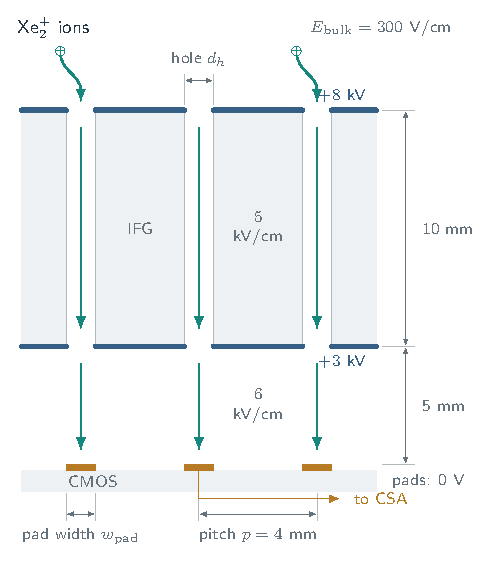
\includegraphics[width=.67\linewidth]{itaca_poo_collection.pdf}
\caption{Ion collection geometry, adapted from the manuscript. The 10 mm IFG
and 5 mm pad gap are drawn in their 2:1 vertical proportion; transverse
features are schematic. Potentials remain 8/3/0 kV. The gate lies upstream
of the drawn IFG.}
\label{fig:concept}
\end{figure}


The closed gate prevents rejected charge from reaching the CSA. Interception
and disposal of blocked ions belong to the gate transport design, so stored
ions are not subsequently counted as a new accepted event. Fixed-potential
electrodes shield the pads from switching; residual aperture coupling can be
bounded by the induced pad charge per unit gate-voltage change. Its magnitude
requires that geometry calculation.

For a 10 mm IFG and 5 mm pad gap, the manuscript's 8/3/0 kV potentials
give nominal fields of 5 and 6 kV/cm respectively. The ion collection
geometry and potentials are retained from the manuscript. At 300 V/cm over 150 cm, the drift voltage difference is 45 kV and
the anode-side drift boundary is 53 kV. An extra transfer gap adds its
specified voltage. At 2 kV/cm/bar, 15 bar and 5 mm EL depth, the EL voltage
difference is 15 kV. The guide grading length is derived from the resulting
exit potential and selected grading field.

Positive ions induce pad current during their final approach. The weighting
potential $\phi_w$ is defined with the selected pad at unit potential and all
other conductors at zero. The biased transport field is a different problem.
For a positive ion, in the adopted input-current sign convention,
\begin{equation}
 i(t)=e\frac{\dd\phi_w(\mathbf r(t))}{\dd t},\qquad
 \int i\,\dd t=e[\phi_w(\mathbf r_f)-\phi_w(\mathbf r_i)].
\end{equation}
Finite-path charge is preserved and the current ends at collection.
Appendix~\ref{app:csa} gives the benchmark pad model and circuit schematics.

The CSA integrates input current and continuously discharges through its
feedback. Its output, including analogue noise, is digitised every
$\Delta t_s=100~\mu$s. Initially the ADC has 12 bits and a 0--1.8 V range;
14 bits and 10 $\mu$s provide comparison settings. Define
$\Delta V=(V_{\max}-V_{\min})/2^B$. An explicit ideal code convention is
\begin{equation}
 c_k=\operatorname{clip}\left(
 \left\lfloor\frac{V_k-V_{\min}}{\Delta V}\right\rfloor,0,2^B-1\right).
\end{equation}
Interior codes can be associated with bin-centre voltages. Simulation records
out-of-range truth separately; the reconstruction interprets endpoint codes
as potentially saturated observations. Transition and endpoint tests specify
this convention.

The device stage ends at codes, timing and calibration metadata. Arrays use
\texttt{UInt16} and compressed HDF5. ADC noise is specified separately from
CSA noise. Analogue input bandwidth and the treatment of noise above Nyquist
are explicit: spectral power is either suppressed by the analogue transfer
or contributes through aliasing. Digital filtering follows digitisation.

\FloatBarrier
\section{Signal treatment}
\subsection{EL channel calibration and SiPM correction}
Subtract the measured pedestal and expected dark contribution, calibrate
single-avalanche charge and account for channel timing and response. The
sensor correction maps measured charge to primary photodetections using its
calibrated recovery model and preceding measured history. PDE and optical
calibration relate that estimate to ionisation charge. Attachment is corrected
using measured drift time and lifetime; residual fluctuations remain.

Sensor compression is invertible where the calibrated response retains
sensitivity. Electronics clipping provides a bound rather than the original
charge. Reconstruction records this distinction. The fast energy estimator
uses corrections compatible with trigger latency; offline processing may
refine them. Each estimator has its own calibrated resolution.

\subsection{Ion baseline, filtering and linear reconstruction}
Pre-arrival ADC samples estimate the starting CSA state and its uncertainty.
An initial 5 ms digital average combines 50 samples. Filter timing, boundary
treatment and gain belong to the calibration. Filtering can work directly in
ADC units, with gain expressed in counts per ion.

For an ideal linear CSA, let $u=V-V_0$ be displacement from its resting voltage:
\begin{equation}
 C_f\dot u+\frac{u}{R_f}=-i(t),\qquad \tau_f=R_fC_f.
\end{equation}
The input charge in a reconstructed bucket is
\begin{equation}
 Q_n=-C_f\left[u(t_n)-u(t_{n-1})+
 \frac1{\tau_f}\int_{t_{n-1}}^{t_n}u(t)\,\dd t\right].
\end{equation}
Measured gain and bandwidth replace the ideal response. Induction and
filtering distribute a deposit between neighbouring buckets; a calibrated
response matrix removes that mixing. Noise covariance passes through the
same operation. Signed reconstructed charge is retained.

\subsection{Nonlinear ion reconstruction}
The existing nonlinear forward model follows $x=V_0-V$ with
\begin{equation}
 \dot x=g(x)\frac{i(t)}e-r(x),
\end{equation}
where $g$ is voltage gain per elementary charge and $r$ the recovery rate.
SPICE calibration uses disjoint fitting and validation histories. This model
predicts voltage; the nonlinear inverse is a separate operation.

The proposed inverse estimates bucket charges and initial state by fitting
the calibrated response to measured ADC history, including noise and
quantisation. The current prescription within each charge bucket is explicit.
Linear and nonlinear estimators receive the same codes. MC truth is reserved
for validation. Any automatic model choice depends on measured response and
the calibration domain. Bias, uncertainty, saturation and fit quality are
reported separately.

\section{Reconstruction of energy and position}
\subsection{Electron track}
Channel coordinates provide transverse positions; corrected electron timing
gives $z=v_e(t_e-t_0)$. The measured distribution has resolution set by
diffusion, hole pitch and signal response. For corrected photodetection
estimates $\widehat n_{cb}$, a schematic energy estimator is
\begin{equation}
 \widehat E_e=K_E\sum_{c,b}
 \frac{\widehat n_{cb}}{\epsilon_{cb}}\exp(t_{e,b}/\tau_e),
\end{equation}
where $\epsilon_{cb}$ is the relative channel/spatial response and $K_E$ the
absolute energy calibration. Corrections already included in $\widehat n$
are applied once. Acceptance and saturation information accompany the sum.

\subsection{Ion track and combined observables}
Pad coordinates and reconstructed collection times give
$z_i=L-v_i(t_i-t_0-\delta_i)$. The measured MARS position transforms local pad
coordinates into the ELM's global transverse frame. The ion charge sum gives
$\widehat E_i=K_i\sum_{p,n}\widehat N_{p,n}$ with its propagated covariance.
The EL branch remains the primary calorimeter.

Each reconstructed track provides a barycentre, longitudinal/transverse
extent, connected components, backbone and endpoint charge. Moments use
consistently corrected weights. Pure MC, diffused and discretised
reconstructions remain distinct validation levels. Comparing the etrack and
itrack in a shared frame tests matching and improves topological information.
Selections and positive-pulse displays are specified separately from signed
charge sums used for energy.

\section{Configuration, storage and validation}
Detector cards specify gas, fields, geometry, lifetime, transport and optics.
Electronics cards specify CSA or SiPM response and readout. Acquisition cards
specify ROI, gate times, channel region and margins. Reconstruction cards
specify filters, estimators and output buckets. Outputs carry units, source
identities, seeds and calibration hashes.

The saved stages are ion counts per pad/bucket and photons per SiPM/bucket;
device response; and reconstructed charge and position. The new ion device
output is ADC codes. Acquisition selects channels from the EL-predicted
detector region or an explicit hardware channel set. Truth-selected pixels
from previous simulations supply a storage benchmark, not a hardware
selection algorithm.

At 100 $\mu$s, each 40 ms interval has 400 samples and occupies 800 bytes per
channel before compression. For $N_p$ channels recorded for $T$ seconds,
payload is approximately $2N_pT/\Delta t_s$ bytes. The short post-arrival
interval reduces storage without waiting for physical feedback recovery.
Pilot measurements establish compression and window sizes before production.

Checks cover charge conservation, ADC transitions and range, reproducibility,
noise spectrum/covariance, temporal convergence and independent SPICE
waveforms. Reconstruction tests compare linear and nonlinear charge recovery
versus intensity, history, timing and saturation. Trigger tests compare
EL-predicted windows with actual ion arrivals and measure excluded charge.
A successive-event test carries the remaining CSA state between accepted
events: gating blocks rejected charge but does not reset admitted charge.

Transport and collection live in \code{src/event_analysis}; electronics in
\code{src/ion_signal}. Existing implementations are documented in
\code{csa_design.tex}, \code{../../docs/ion_csa_nonlinear_model.html}, and
\code{../../docs/sipm_statistical_implementation.md}. Julia calculates and
saves numerical results to HDF5; Python generates report figures and tables.
This note defines the new operating model before implementation.

\appendix
\section{CSA geometry, circuit and response details}
\label{app:csa}
Figure~\ref{fig:equivalent} shows the equivalent pixel circuit and ADC readout.
Figure~\ref{fig:csa} gives the transistor schematic supplied by Rogelio Palomo.
\begin{figure}[htbp]\centering
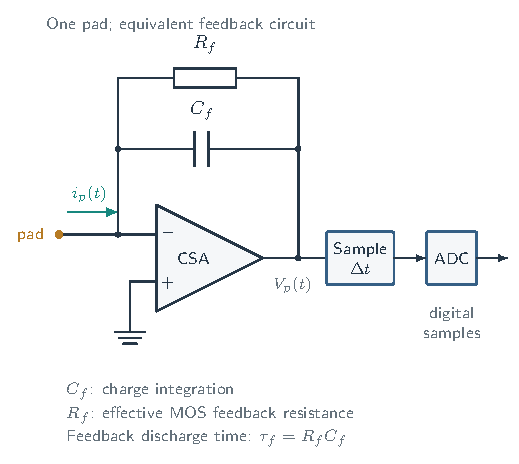
\includegraphics[width=.80\linewidth]{itaca_poo_circuit.pdf}
\caption{Equivalent CSA circuit and digitised readout, adapted from the
manuscript. The effective resistance represents the MOS feedback discharge.}
\label{fig:equivalent}
\end{figure}
\begin{figure}[htbp]\centering
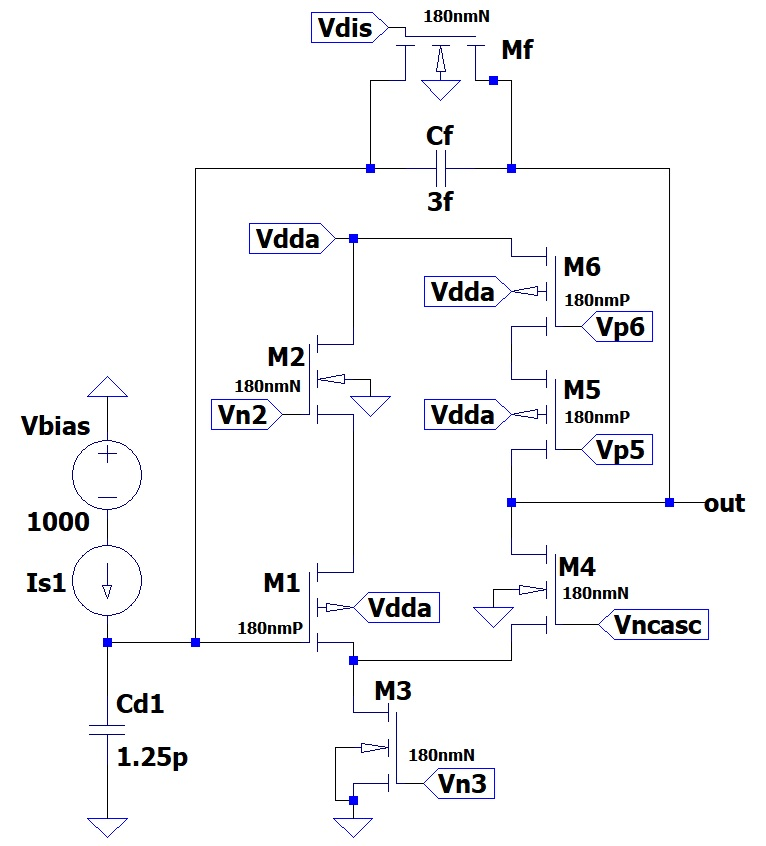
\includegraphics[width=.70\linewidth]{Nausica_Image.jpg}
\caption{CSA transistor schematic reused from the ITACA manuscript and CSA
note. The pad drives the input transistor; $C_f$ integrates charge and the
feedback transistor supplies the discharge path.}
\label{fig:csa}
\end{figure}
The calibrated 180 nm circuit uses a 1.8 V supply, $C_f=3$ fF and external
input capacitance 1.25 pF. Its resting output is approximately 0.886 V and
small-signal decay time approximately 19.5 s. Dimensions and biases are in
\code{csa_design.tex} and its generated tables. A circuit change requires
revalidation.

For the square-pad benchmark of half-width $a$ in a grounded plane,
\begin{equation}
 \phi_w(z)=\frac2\pi\tan^{-1}\frac{a^2}{z\sqrt{z^2+2a^2}},\qquad
 W(z)=-\phi_w'(z)=\frac{4a^2}{\pi(z^2+a^2)\sqrt{z^2+2a^2}}.
\end{equation}
An ion approaching at speed $v$, collected at $t=0$, gives
$i_1(t)=evW(-vt)$ over $-g/v\leq t<0$. Its integral is
$e[1-\phi_w(g)]$, following the weighting-field prescription~\cite{riegler2016}.
The manuscript contains the square-pad derivation. The actual perforated
electrodes and dielectrics define the eventual detector weighting solution.

For one-sided output-noise spectrum $S_V(f)$ and linear measurement filter
$H(f)$, variance is $\int S_V(f)|H(f)|^2\dd f$. Earlier calculations combine
averaging and frame subtraction before sampling reconstructed noise. The new
ADC model samples voltage noise before quantisation, then applies digital
reconstruction. Compression can retain information; actual saturation loses
it. The inverse must distinguish these behaviours.

\section{SiPM microcells and readout details}
\label{app:sipm}
The current optical design illuminates a centred 2.5 mm disk on a
$3\times3$ mm$^2$ Hamamatsu S14160-3015PS with 15 $\mu$m cells. Its card uses
39,984 total and 21,808 illuminated cells, gain $3.6\times10^5$ and PDE 0.32
as a provisional blue-spectrum average~\cite{HamamatsuS14160SmallCells}.
The 12.5 ns exponential recovery constant is provisional, with 25 ns as a
sensitivity case.

Photodetections are binomial samples of incident photons with probability
PDE. A cell firing $\Delta t$ after its preceding avalanche contributes
\begin{equation}
 q=q_0[1-\exp(-\Delta t/\tau_s)],\qquad q_0=eG.
\end{equation}
Its state persists between buckets. Dark triggers also change recovery; the
current card takes a 700 kHz total dark rate at its reference operating point.
Crosstalk, afterpulsing and gain spread are disabled in that baseline.

The statistical model carries the sum of recovery fractions and their
squares. Sparse buckets use individual trigger times; denser ones use
substeps and finite-cell occupancy moments. Illuminated and dark-only cell
populations retain their identities. The implementation and reference tests
are described in \code{../../docs/sipm_statistical_implementation.md}.

Under steady uniform illumination of $M$ participating cells, expected trigger
count $n$ over duration $T$ gives mean PE-equivalent charge
\begin{equation}
 m=\frac{n}{1+kn},\qquad k=\frac{\tau_s}{MT},\qquad
 n=\frac{m}{1-km}.
\end{equation}
This AXEL-related mean correction~\cite{Ban2020AXELPrototype} is a limiting
case and calibration check. Transient correction uses preceding measured
history. The inverse becomes poorly conditioned near the asymptote.

The provisional readout converts charge to bucket-average current $I=Q/T$,
adds 0.5 PE-equivalent RMS independent electronics noise per 250 ns bucket
and limits output at 1 mA. These are card-selected assumptions. A change of
bucket duration requires consistent electronics noise and transfer settings.
Dark fluctuations are separate from electronics noise. Sensor charge saved
before electronics permits that stage to be regenerated independently.

\bibliographystyle{unsrt}
\bibliography{references}
\end{document}
